\documentclass[titlepage,11pt]{article}

\textwidth 6.5in
\textheight 9in
\oddsidemargin -0.2in
\topmargin -0.5in

\usepackage{indentfirst,graphics,alltt,epsfig,color}

\title{iBioSim: Tutorial}

\author{Chris J. Myers}

\date{Created: August 11th, 2008\\
  Last Revised: August 11th, 2008
}

\begin{document}

\maketitle

%show only subsection granularity in the toc
%\setcounter{tocdepth}{2} 
  
\tableofcontents

\clearpage
  
%\setlength{\parindent}{0em}
%\setlength{\parskip}{10pt}

\section{Introduction}

The example described in this tutorial constructs a simple model for
the \emph{cI} and \emph{cII} genes and the $P_R$ and $P_{RE}$
promoters from the phage $\lambda$ decsion circuit.  This example
illustrates many of the features of {\tt iBioSim}.

% TODO: add figures and more description of the example

\section{SBML Editor}

\noindent
After starting {\tt iBioSim}, complete the following steps to create
an SBML model for this example:
\begin{enumerate}
\item Select {\tt File} $\rightarrow$ {\tt New} $\rightarrow$ {\tt Project}.
      Browse to desired path and create a project named {\tt demo}.

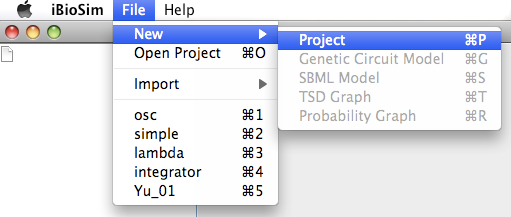
\includegraphics[height=50mm]{screenshots/project}

\item Select {\tt File} $\rightarrow$ {\tt New} $\rightarrow$ {\tt SBML Model}.
      Enter {\tt lambda} as the SBML model ID at which point an SBML
      editor will open.

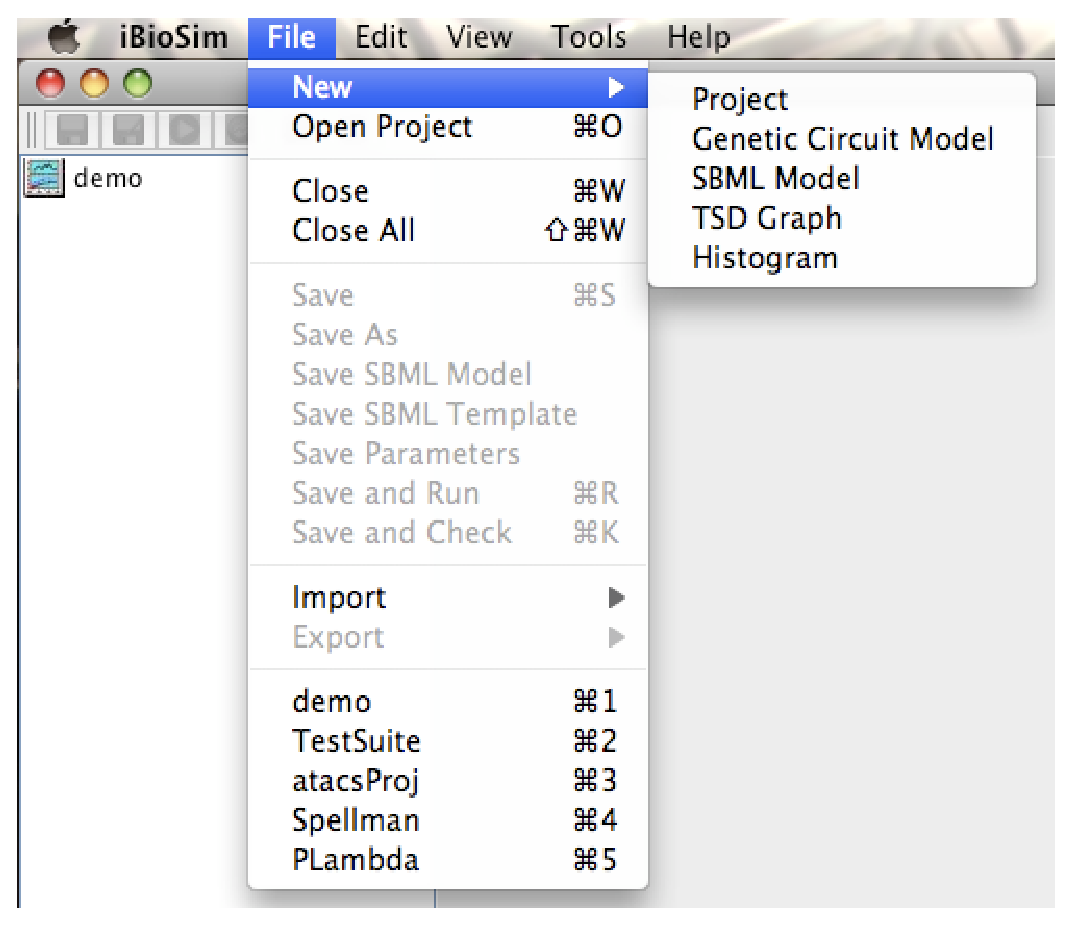
\includegraphics[height=45mm]{screenshots/newModel}

\item Select {\tt Edit Compartment} and change ID from {\tt default} 
to {\tt Cytoplasm}.  Also, change Units to {\tt volume}.

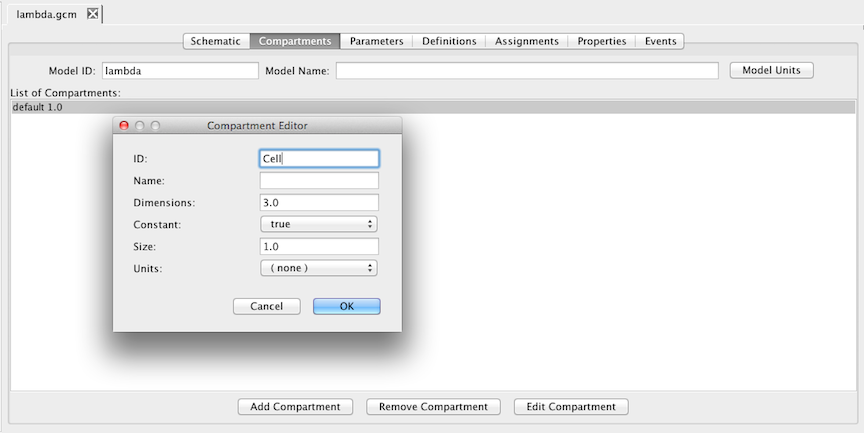
\includegraphics[height=70mm]{screenshots/compartment}

\item Select {\tt Add Species} and enter {\tt CI} as the ID, 
{\tt The lambda repressor} as the name, and change the units 
to {\tt mole}.  Select {\tt Add Species} again and enter {\tt CI2} as the ID,
{\tt CI dimer} as the name, and change the units to {\tt mole}.

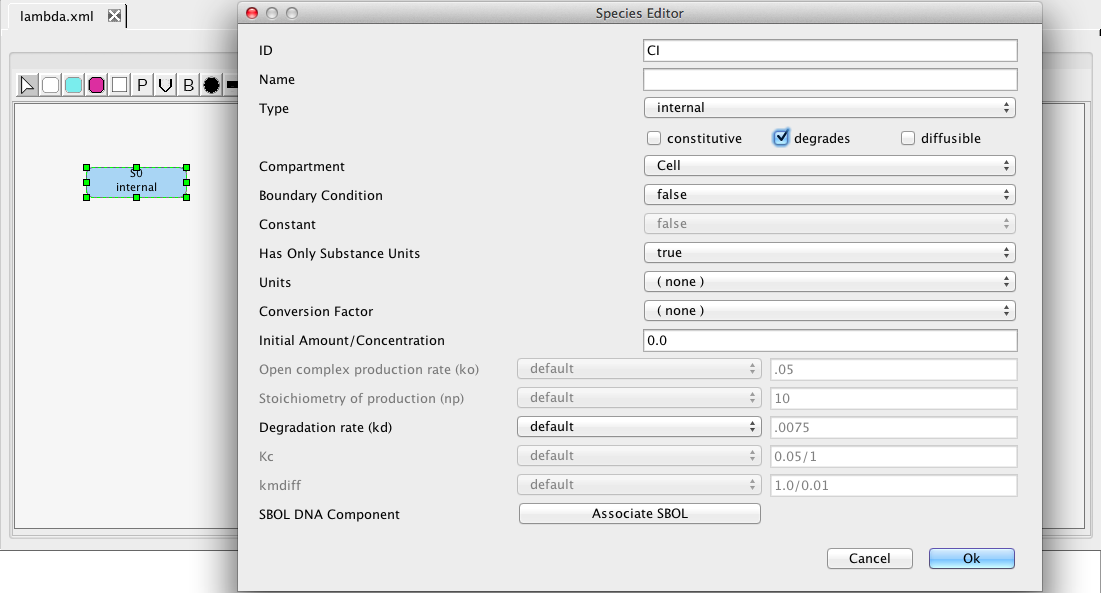
\includegraphics[height=70mm]{screenshots/species}

\item Select {\tt Add Parameter} and enter {\tt nd} as the ID,
      {\tt Number of molecules in dimer} as the name, and change the
      units to {\tt dimensionless}.

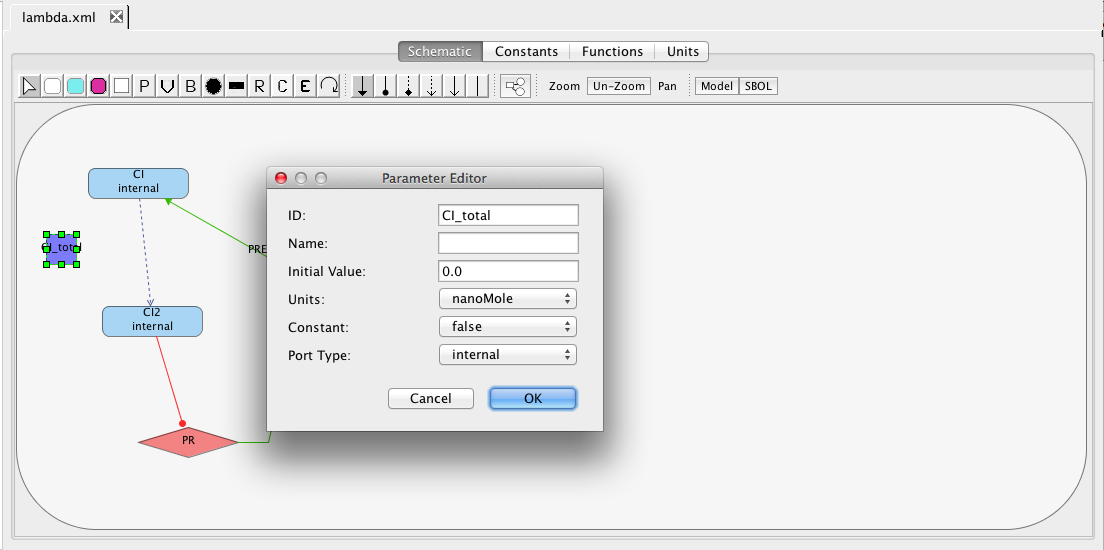
\includegraphics[height=60mm]{screenshots/parameter}

\item Select {\tt Definitions/Types} tab, and select {\tt Add Unit}
      and enter {\tt per\_second} as the ID.  Select {\tt Add to List}, 
      select {\tt second} as the kind, change the exponent to $-1$, 
      and click {\tt Add}.  Click {\tt Add} in the {\tt Unit Definition Editor}.
      Repeat these steps to create a {\tt per\_second\_mole} unit 
      (i.e., (second)$^{-1}$(mole)$^{-1}$).

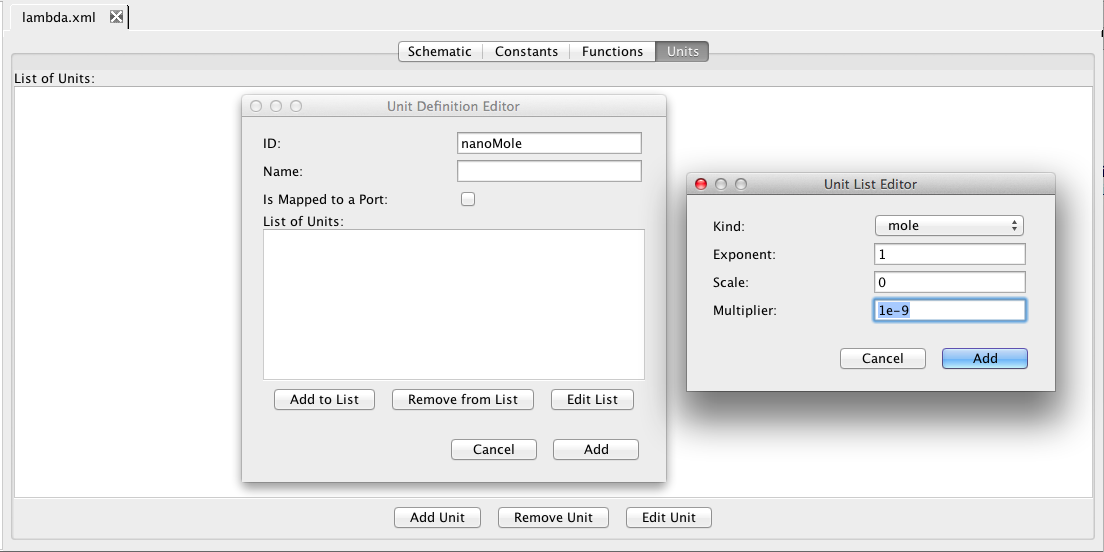
\includegraphics[height=75mm]{screenshots/units}

\item Select {\tt Main Elements} tab.  Select {\tt Add Reaction} and
  enter {\tt Dimerize\_CI} as the ID, {\tt Reaction to dimerize CI} as
  the name, and change reversible to {\tt true}.

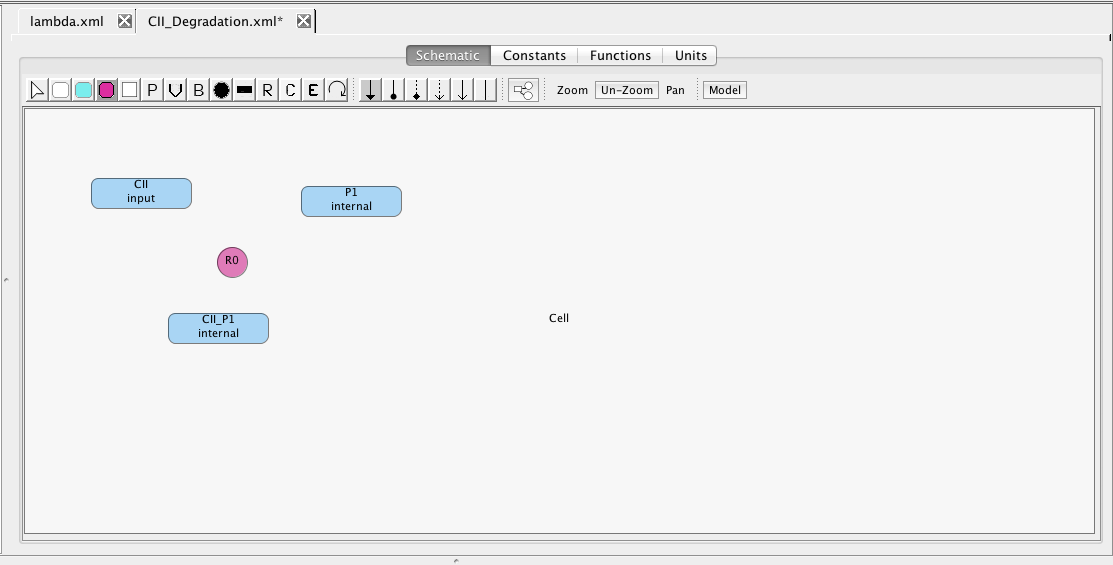
\includegraphics[height=70mm]{screenshots/reaction}

\item Select {\tt Add Reactant} and select {\tt CI} as the species,
      {\tt Stoichiometry} to {\tt Stoichiometry math}, and set its
      value to {\tt nd}.

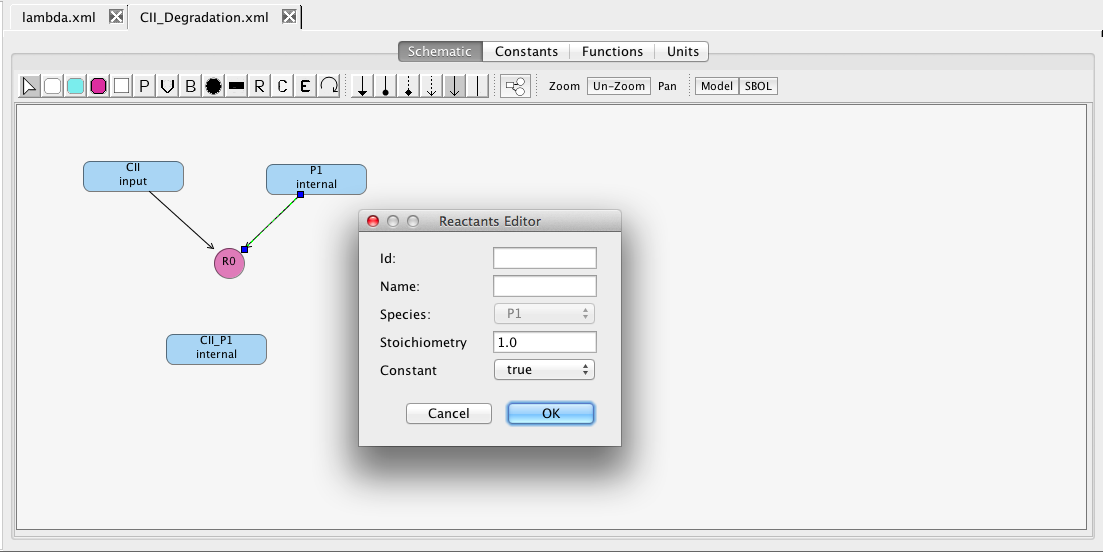
\includegraphics[height=60mm]{screenshots/reactant}

\item Select {\tt Add Product} and select {\tt CI2} as the species.
      Leave the stoichiometry as 1.

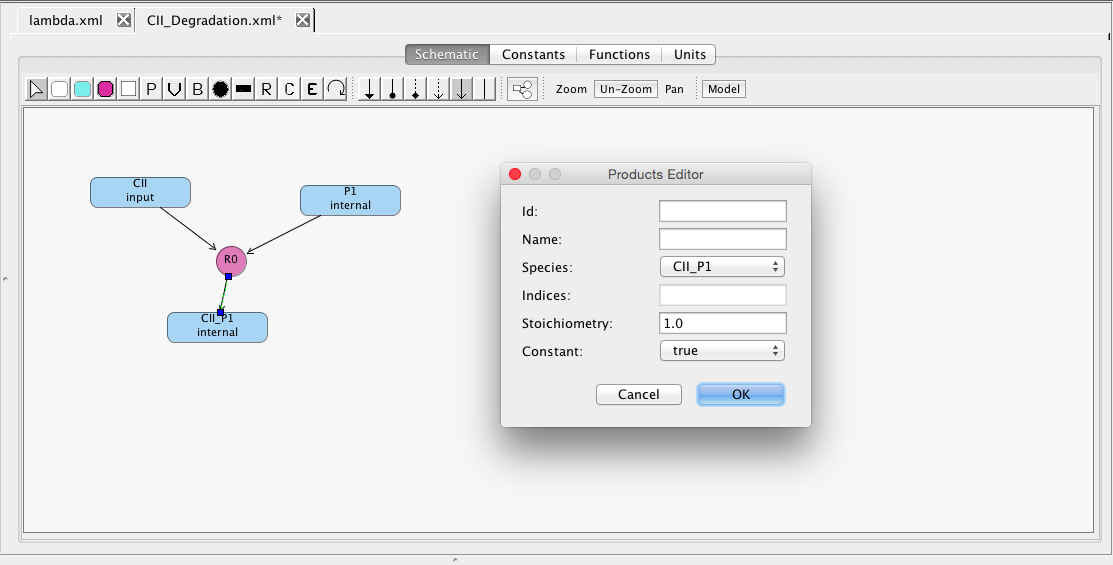
\includegraphics[height=60mm]{screenshots/product}

\item Highlight {\tt kf} and select {\tt Edit Selected Parameter}, change
      {\tt kf} to {\tt k2f}, and change the units to {\tt per\_second\_mole}.
      Highlight {\tt kr} and select {\tt Edit Selected Parameter}, change
      {\tt kr} to {\tt k2r}, and change the units to {\tt per\_second}.

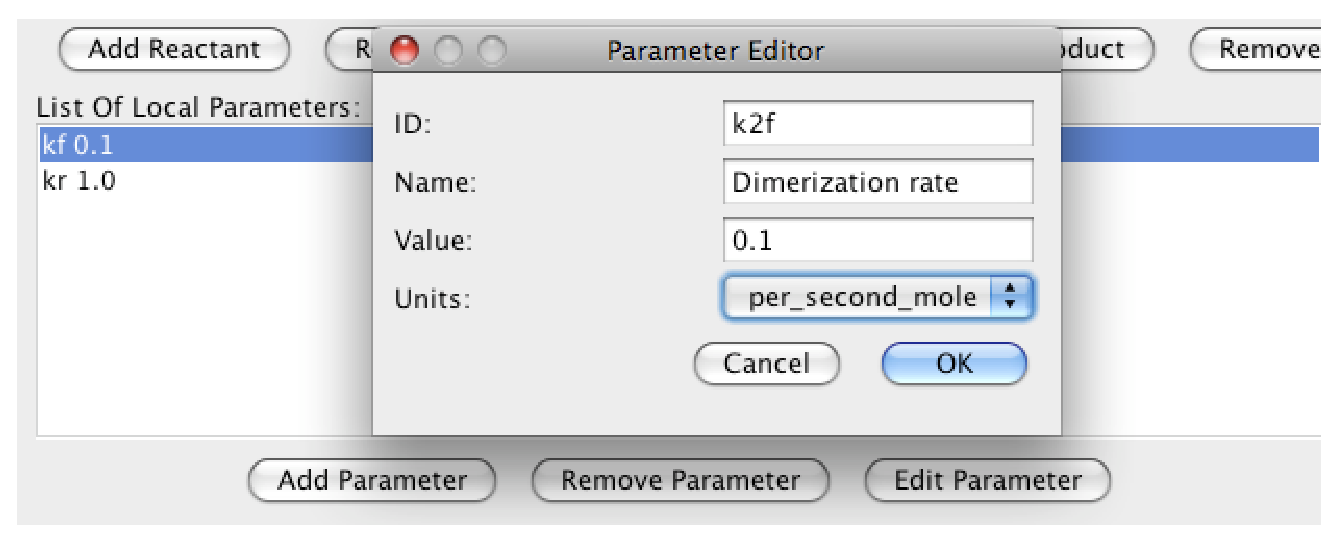
\includegraphics[height=60mm]{screenshots/localParam}

\item Select {\tt Use Mass Action}, select {\tt Add}, 
      and select {\tt Save and Check SBML}.  There should be no errors.

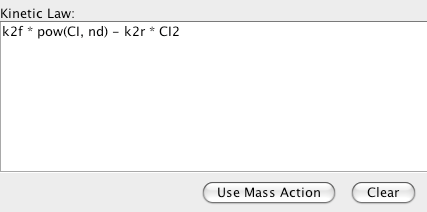
\includegraphics[height=60mm]{screenshots/kineticLaw}

\item Add a new species ``CI\_total'' with units of {\tt mole}.
      Click on the ``Initial Assignments/Rules/Constraints/Events'' tab
      and press the ``Add Rule'' button.
      Select Assignment Type, select Variable ``CI\_total'', 
      and enter the following as the Rule:
\begin{eqnarray*}
& 2 * CI2 + CI &
\end{eqnarray*}

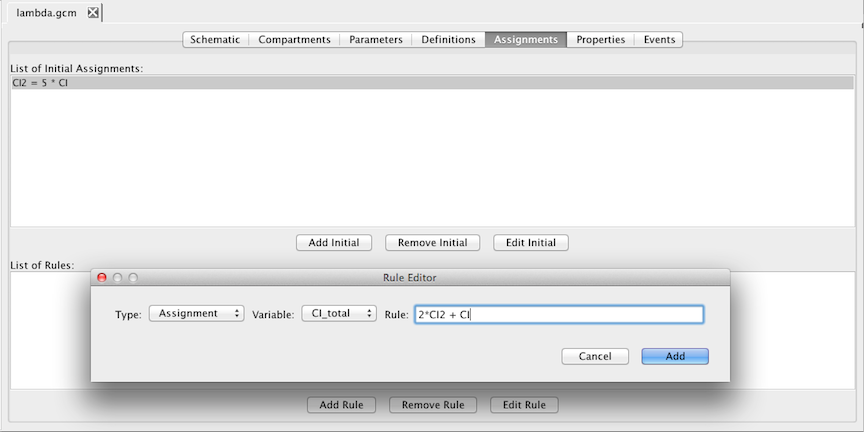
\includegraphics[height=60mm]{screenshots/rule}

\item Highlight {\tt lambda.sbml}, using right mouse button, select 
      {\tt View Network}.
      Highlight {\tt lambda.sbml}, using right mouse button, select 
      {\tt View in Browser}.

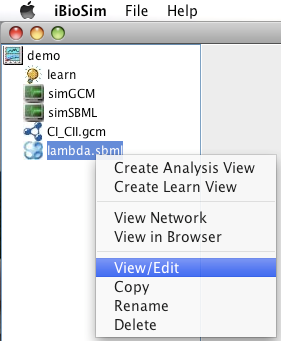
\includegraphics[height=74mm]{screenshots/modSBML}

\item Go back to the SBML editor complete the construction of the
      chemical reaction network shown below:
\begin{eqnarray*}
PRE + \mathrm{RNAP} & \stackrel{KPRE2}{\longleftrightarrow} &
PRE\_\mathrm{RNAP} \\
PRE + \mathrm{CII} + \mathrm{RNAP} &
\stackrel{KPRE4}{\longleftrightarrow} &
PRE\_\mathrm{CII}\_\mathrm{RNAP} \\
PRE\_\mathrm{RNAP} & \stackrel{kPREb}{\longrightarrow} & 
PRE\_\mathrm{RNAP} + n\mathrm{CI} \\
PRE\_\mathrm{CII}\_\mathrm{RNAP} 
& \stackrel{kPRE}{\longrightarrow} & 
PRE\_\mathrm{CII}\_\mathrm{RNAP} + n\mathrm{CI} \\
PR + \mathrm{RNAP} & \stackrel{KOR9}{\longleftrightarrow} &
PR\_\mathrm{RNAP} \\
PR + 2 \mathrm{CI2} & \stackrel{KOR10}{\longleftrightarrow} &
PR\_2 \mathrm{CI2} \\
PR\_\mathrm{RNAP} & \stackrel{kPR}{\longrightarrow} & 
PR\_\mathrm{RNAP} + n\mathrm{CII} \\
2 \mathrm{CI} & \stackrel{K2}{\longleftrightarrow} & \mathrm{CI2} \\
\mathrm{CI} & \stackrel{k1}{\longrightarrow} & () \\ 
\mathrm{CII} & \stackrel{k10}{\longrightarrow} & ()
\end{eqnarray*}

\begin{center}
\begin{math}
\begin{array}{|c|c|c|c|c|c|c|c|}
\hline
Constant & Value & Constant & Value &
Constant & Value & Constant & Value \\ \hline \hline
KPRE2  & 0.01~M^{-1} & KPRE4  & 0.00161~M^{-2} & 
kPREb  & 0.00004~\mathrm{sec}^{-1} & 
kPRE   & 0.015~\mathrm{sec}^{-1} \\ \hline
n         & 10 & KOR9  & 0.69422~M^{-1} & KOR10  & 0.06568~M^{-2} &
kPR    & 0.014~\mathrm{sec}^{-1} \\ \hline
K2       & 0.1 M^{-1} & k1       & 0.0007~\mathrm{sec}^{-1} &
k10    & 0.002~\mathrm{sec}^{-1} & ~ & ~ \\ \hline
\end{array}
\end{math}
Set an initial amount of 1.0 for PRE and OR, 30.0 for RNAP, and 0.0 
for the rest.
\end{center}
\end{enumerate}

\section{Analysis}

The following instructions describe how to analyze the SBML file just 
created.
\begin{enumerate}
\item Highlight {\tt lambda.sbml}, using the right mouse button, select 
      {\tt Create Analysis View}, and enter the name {\tt sim}.

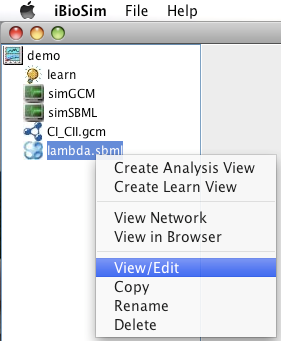
\includegraphics[height=74mm]{screenshots/modSBML}

\item In the newly opened window, select {\tt Monte Carlo}.
      Also, in this window, change the time limit to 2100.0, print interval
      to 100.0, and runs to 20.
      Finally, select {\tt Save and Run} at the bottom of the window.

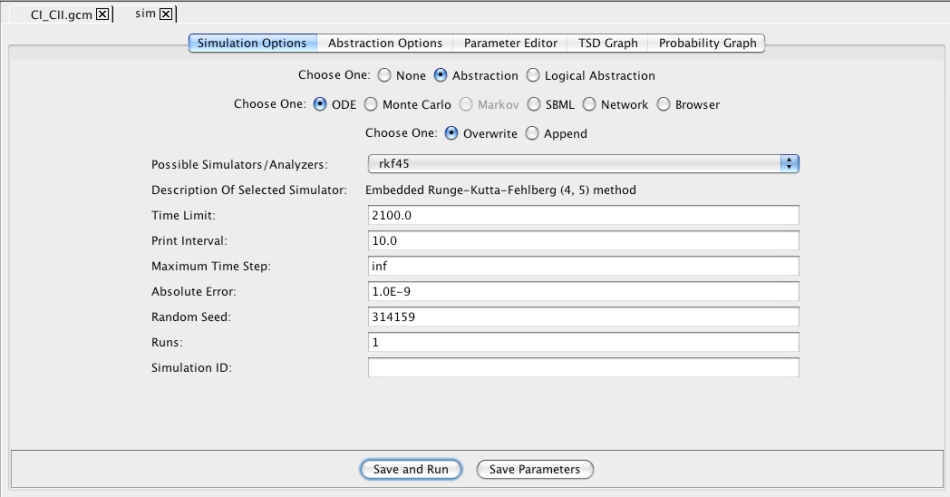
\includegraphics[height=80mm]{screenshots/analysisView}

\item After the simulation completes (it may take a little while), click on
      the graph tab.

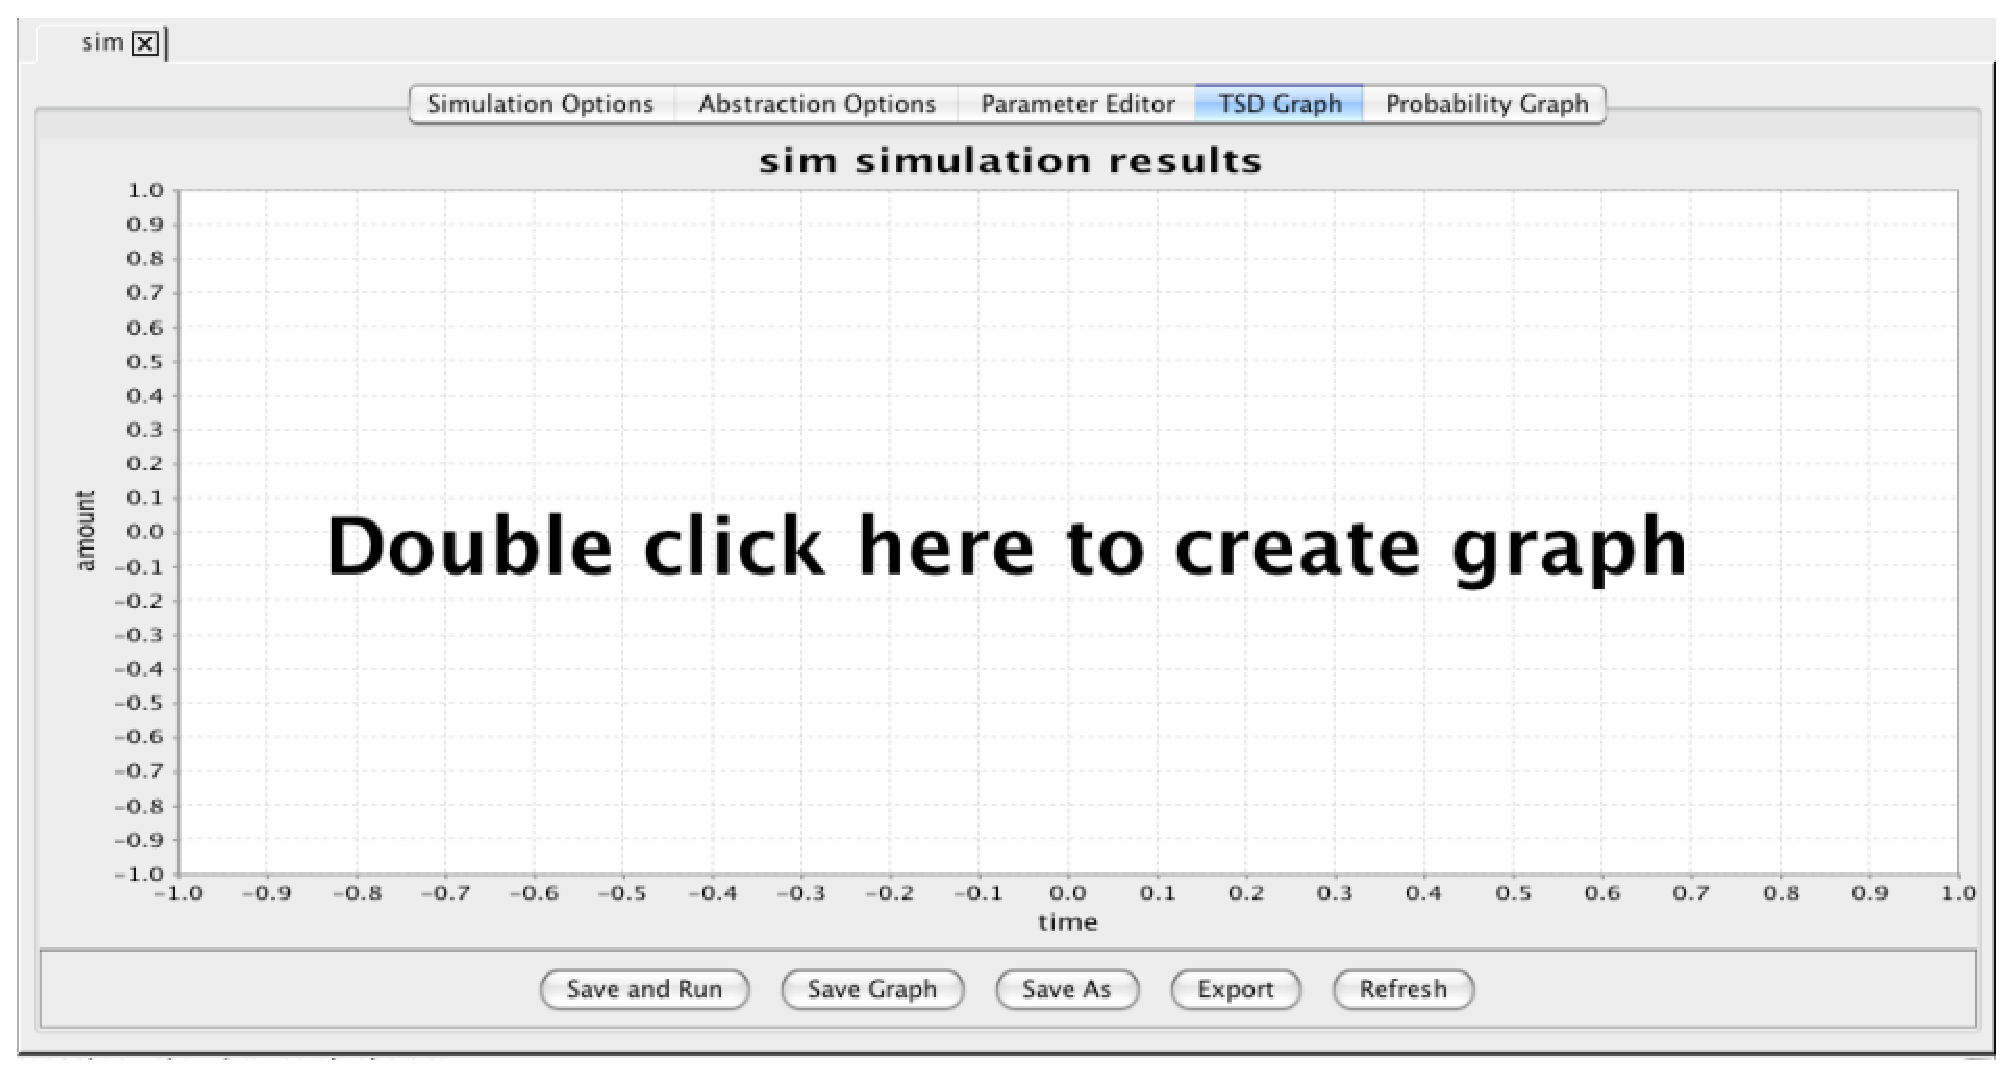
\includegraphics[height=60mm]{screenshots/emptyGraph}

\item Click on the graph to bring up the graph editor.  Highlight Average,
      if not already highlighted, select CI2 and CII, change Title to
      ``Average'', change X-Axis Label to ``Time (seconds)'', and change
      Y-Axis Label to ``Number of Molecules''.  Press the OK button.
      Click on Export and enter file name of {\tt average.jpg}.
      Repeat these steps to generate graphs for the standard deviation
      {\tt stddev.jpg} and run-1 {\tt run1.jpg}.  
      Note that you can use the ``Deselect All'' button to
      remove all items from the graph.

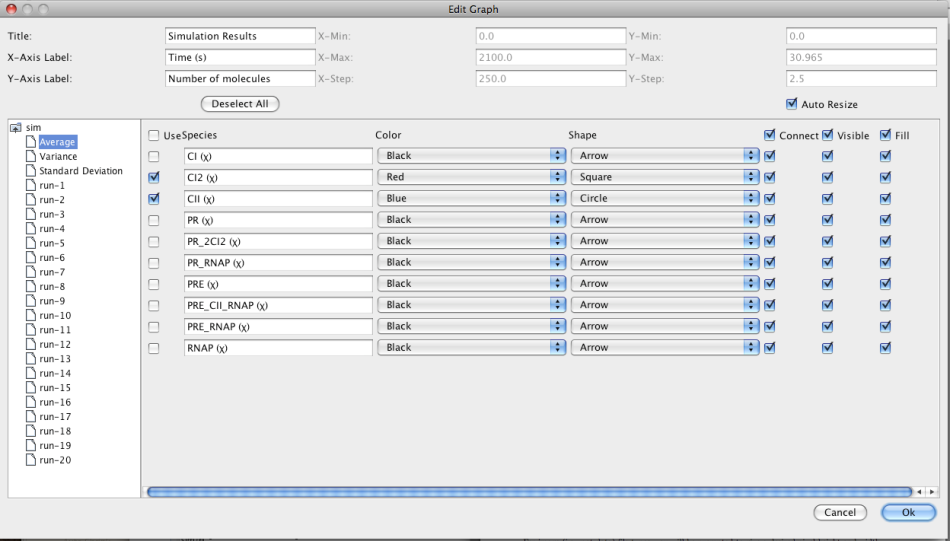
\includegraphics[height=70mm]{screenshots/editGraph}

\item Click on the SBML editor tab.  Change the initial amounts of OR and
      PRE to 10.  Press the Save and Run button.
      Click on the graph tab and following the steps above, create the 
      following plots {\tt average\_10.jpg},  {\tt run1\_10.jpg}, and
      {\tt stddev\_10.jpg}.  

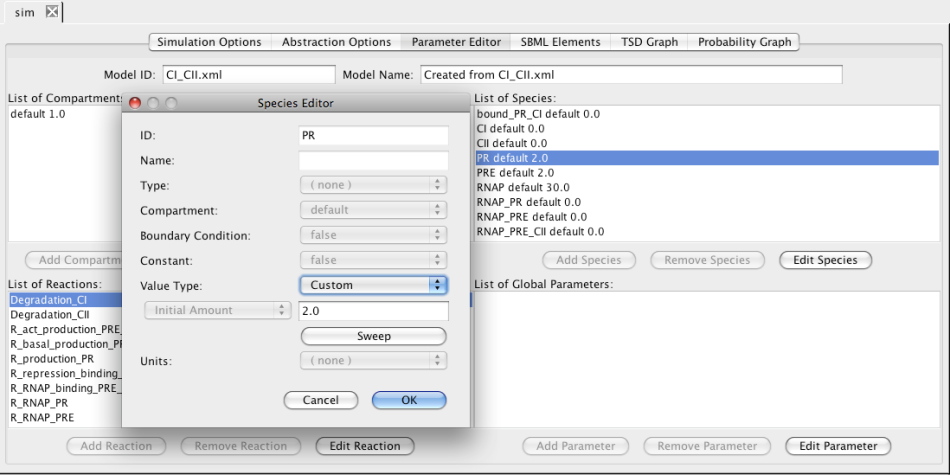
\includegraphics[height=70mm]{screenshots/paramEdit}

\item Simulate your lambda model with BioSim using the ODE method rkf45 with
      a time limit of 2100 and print interval of 50.
      Make a note of the simulation time and plot CI2 and CII.  
      Next, simulate using the Euler method.  Make a note of the simulation time
      and add CI2 and CII from the euler results to your graph.  
      How do the simulation times and results compare?
      Change the time step and rerun the Euler method.  Repeat until the results
      match up well.  What time step is required for a good match?
      How do the simulation times compare?
\end{enumerate}

\section{Abstraction}

The example in this section illustrates abstraction-based synthesis. 
\begin{enumerate}
\item Press the Save SBML button.

\item Create or open an analysis view on your lambda model.

\item Select ``None'' and ``Network'', and press the Save and Run button. 
      Count the number of species and reactions in your model.  

\item Select ``Monte Carlo'', set the Time Limit to 2100.0, Print Interval to
      100.0, and Runs to 20.  Press the Save and Run button and record the
      simulation time.

\item Create a new analysis view for your lambda model and 
      select  ``Abstraction'' this time.  

\item In the abstraction tab, change rapid equilibrium conditions 1 and 2 
      to 1000.0 as well as QSSA condition to 1000.0.  Select ``Network'' then 
      save and run.  Count the number of species and reactions in your model.

\item Select ``Monte Carlo'', set the Time Limit to 2100.0, Print Interval to
      100.0, and Runs to 20.  Press the Save and Run button and record the
      simulation time.

\item Select File $\rightarrow$ New $\rightarrow$ Graph and enter a name for
      your new top-level graph.

\item Click on the graph and find the average simulation results from your
      orginal model and graph CII and CIt.  Also, add to this graph from
      your abstracted model CII and CI.  How well do they compare?  
      Send me by email a jpg of your result.

\item Go back to your analysis view in which you did abstraction and change
      all the conditions back to 0.1.  Regenerate the network and record the
      number of species and reactions.  Regenerate the simulation results and
      record the simulation time.  

\item Go back to the top-level graph which should have updated results.  
      How does it compare now?
\end{enumerate}

\section{GCM Editor}

This section gives an example using the GCM editor.
\begin{enumerate}
\item Create a new project named ``xor'',
      select File $\rightarrow$ New $\rightarrow$ Genetic Circuit Model, 
      and enter the name {\tt xor}.

\item Add species $A$ and $B$ of type constant.  Be sure to fill in both
      the ID and Name fields.

\item Add species $Abar$, $Bbar$, $X$, $Y$, and $C$ of type normal.  Again,
      fill in the ID and Name fields.

\item Add an influence of type repression with input $A$ and output $Abar$ and 
      dimer of 2.  You have just created an inverter.
      Create another inverter from $B$ to $Bbar$.

\item Add a promoter named PX1 and another promoter named PX2.

\item Add a repression influence from $A$ to $X$ and use the promoter 
      PX1 with dimer of 2.

\item Add a repression influence from $Bbar$ to $X$ and use the promoter 
      PX2 with dimer of 2.  You have just created a NAND gate.

\item Create another NAND gate with inputs $Abar$ and $B$ and output $Y$.

\item Finally, create another NAND gate with inputs $X$ and $Y$ and 
      output $C$.

\item Change the {\tt decay} parameter to 0.01.

\item Press the ``Save GCM'' and ``Save as SBML'' buttons.

\item Create an analysis view for your {\tt xor.sbml} file.

\item Select the User Defined Data tab and click on the 
      ``Use User Defined Data'' button.

\item Add a data point for A at time step 1000 to go to 20.

\item Add a data point for B at time step 2000 to go to 20.

\item Add a data point for A at time step 3000 to go to 0.

\item Add a data point for B at time step 4000 to go to 0.

\item Select the options tab, select ``abstraction'', and 
      set a time limit of 5000, a print interval of 200, and 20 runs.  

\item Select the abstraction tab, and add species $C$ to the interesting 
      species list.

\item Press the ``Save Parameters'' button then ``Save and Run'' button.

\item Create a graph that includes $A$, $B$, and $C$.  Email a jpg
      of this graph to me.

\item Close your analysis view and edit your {\tt xor.gcm}.  Try adjusting
      some of the global parameters.  Remember to save both your {\tt gcm}
      {\tt sbml} files.  Reopen your analysis view and re-run your simulation.
      Send me a few different graphs.  Change the titles of the graphs 
      and provide a description in your email of the graphs as to what you
      changed.
\end{enumerate}
  
\end{document}